\documentclass[a4paper, 12pt]{article}
\usepackage[utf8]{inputenc}
\usepackage[american]{babel}
\usepackage[margin=1in]{geometry}
\usepackage{mathtools}
\usepackage{fancyhdr}
\usepackage{tikz}
\usepackage{enumitem}
\usetikzlibrary{shapes, calc}
\setlength{\headheight}{15.2pt}
\pagestyle{fancy}
\lhead[]{Joseph Petitti}
\rhead[]{Homework 4}
\chead[]{Database Systems II}

\begin{document}

\section*{Problem 1}

\begin{enumerate}[label=\textbf{S\arabic*:}]
	\item 
		\begin{enumerate}[label=Q\arabic*:]
			\item Precedence graph: \\
				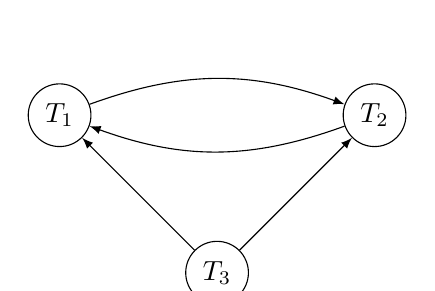
\begin{tikzpicture}[
						every node/.style={circle, draw},
						every path/.style={>=latex}]
					\node (T1) at (0,0) {$T_1$};
					\node (T2) at (4,0) {$T_2$};
					\node (T3) at (2,-2) {$T_3$};

					\path [->] (T1) edge [bend left=20] (T2);
					\path [->] (T3) edge (T2);
					\path [->] (T3) edge (T1);
					\path [->] (T2) edge [bend left=20] (T1);
				\end{tikzpicture}
			\item This schedule is not conflict-serializable because the
				precendence graph for the schedule is cyclic.
		\end{enumerate}

	\item 
		\begin{enumerate}[label=Q\arabic*:]
			\item Precedence graph: \\
				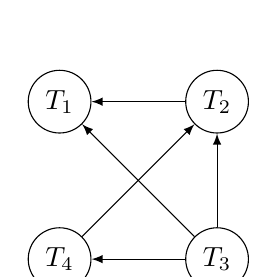
\begin{tikzpicture}[
						every node/.style={circle, draw},
						every path/.style={>=latex}]
					\node (T1) at (0,0) {$T_1$};
					\node (T2) at (2,0) {$T_2$};
					\node (T3) at (2,-2) {$T_3$};
					\node (T4) at (0,-2) {$T_4$};

					\path [->] (T3) edge (T1);
					\path [->] (T3) edge (T2);
					\path [->] (T3) edge (T4);
					\path [->] (T2) edge (T1);
					\path [->] (T4) edge (T2);
				\end{tikzpicture}
			\item This schedule is conflict-serializable because the precendence
				graph for the schedule is acyclic. An equivalent serial schedule
				would be $T_3, T_4, T_2, T_1$.
		\end{enumerate}
	
	\item
		\begin{enumerate}[label=Q\arabic*:]
			\item Precedence graph: \\
				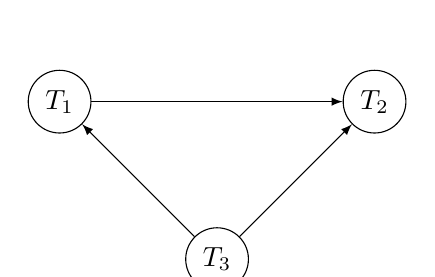
\begin{tikzpicture}[
						every node/.style={circle, draw},
						every path/.style={>=latex}]
					\node (T1) at (0,0) {$T_1$};
					\node (T2) at (4,0) {$T_2$};
					\node (T3) at (2,-2) {$T_3$};

					\path [->] (T3) edge (T1);
					\path [->] (T1) edge (T2);
					\path [->] (T3) edge (T2);
				\end{tikzpicture}
			\item This schedule is conflict-serializable because the precendence
				graph for the schedule is acyclic. An equivalent serial schedule
				would be $T_3, T_1, T_2$.
		\end{enumerate}
\end{enumerate}

\section*{Problem 2}

\begin{enumerate}[label=Q\arabic*:]
	\item $S_1$ is not a valid schedule, because in the fifth action $T_2$ tries
		to lock object B while $T_1$ already has a lock on it.

		$S_2$ is not a valid schedule, because in the fifth action $T_1$ tries
		to unlock object B, when it does not own a lock for object B.
	\item $T_1$ in $S_1$ is well-formed, because all of its read/write actions
		are performed after locking the object and before unlocking the object.

		$T_1$ in $S_2$ is not well-formed, bceause in the third action it tries
		to write to object B before it has a lock on that object.
\end{enumerate}

\section*{Problem 3}

This sequence follows 2PL, because neither transaction performs an unlock before
it has all its locks.

\section*{Problem 4}

\begin{enumerate}[label=(\alph*)]
	\item Undo \texttt{<T, A, 10>} by setting A to 10.
\end{enumerate}

\end{document}
